% -*- root: ../linear-systems-notes.tex -*-

\chapter{Signals and Systems}

% \begin{chapquote}{Author's name, \textit{Source of this quote}}
% ``This is a quote and I don't know who said this.''
% \end{chapquote}

\section{What is a signal?}
A \textit{signal} is defined as any measurable physical quantity carrying information that depends on one or more independent variables, such a time, space etc. Mathematically, a signal can be represented a function of a set of independent variable(s). For example,
\[ s\ct{t} = 0.23t^2 - 5.11t + 31.5 \]
where, $t$ is time. This is an example ofa  1-dimensional (1-D) signal, i.e. a signal that is a function of a single independent variable. 

\begin{figure}[h]
\centering
    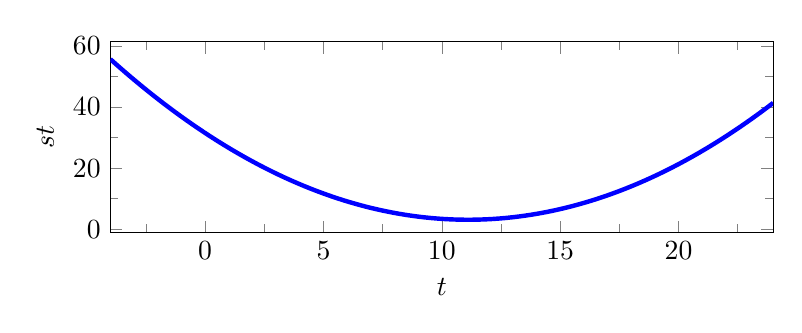
\begin{tikzpicture}[scale=1.0]
        \begin{axis}[xmin=-4,
        xmax=24,
        ymin=-1.0,
        samples=100,
        grid style={line width=.1pt, draw=gray!10},
        major grid style={line width=.2pt,draw=gray!50},
        minor tick num=1,
        xlabel={{$t$}},
        ylabel={{$s\ct{t}$}},
        title={},
        width=10cm,
        height=4.0cm]
        \addplot[blue, ultra thick, domain=-4:24](x, 0.23*x*x - 5.11*x + 31.5);
    \end{axis}
    \end{tikzpicture}
\caption{Visualization of a 1-D signal} \label{fig:ch1_signal_1d}
\end{figure}

An image is a 2-D signal that is a function of two independent spatial variables $x$ and $y$. In the case of a gray-scale image, the intensity of the image at a spatial location is given by $I\ct{x, y}$, where $x$ is horizontal position, and $y$ is the vertical position.

A mathematical representation a signal is not always possible for all types of signals. For example, many of the physiological signals cannot be represented mathematically, either because the exact function is not known or is too complicated.

\begin{problem*}[frametitle=Higher dimensional signals]
    Can you think of an examples of a 3-D and 4-D signals?
\end{problem*}

\section{Classification of signals}

A particular type of signal classification was already mentioned in the previous section, based on the number of independent variables associated with the signal. Some of the other common classifications of signals are described in this section.

\subsection{Scalar and Vector Signals}

Signals can take one or more values for each value(s) of its independent variables. \textit{Scalar} signals take on only one value, while \textit{vector} signals take more than one value. A gray-scale image is an example of a scalar 2-D signal, while a RGB image is an example of a vector 2-D signal (with each point on the image taking three values). 
\[ I\left(x, y\right) \in [0, 1] \]
where, $I\left(x, y\right)$ is the intensity of the point with 0 corresponding to black and 1 corresponding to white colors. An RGB image on the other hand can be represented as the following,
\[ \mathbf{I}\ct{x, y} = \bmx r & g & b \emx^{T} \]
where, $r, g, b \in [0, 1]$ correspond to the amount of red, green and blue components at each point in the image. The different combinations of these three primary colors results in the different colors in the image.

\subsection{Continuous-time and Discrete-time Signals}

An important classification of signals is based on the nature of the values assumed by the independent variable of a signal. \textit{Continuous-time} signals are ones whose independent variable can take on any value in continuous interval $\left(a, b\right)$ on the real axis. For example, a function $e^{-0.1t^{2}}$ with $t \in \left(-\infty, \infty\right)$ is an example of a continuous-time signal. 

On the other hand, \textit{discrete} signals can take on values only for specific values of the independent variable. They can be represented in a tabular form that represents the mapping from the signal's domain to its range. For example consider a discrete signal $x\dt{t}$ that takes on values only for specific time instants $t \in \lc \ldots, t_{n}, t_{n+1}, t_{n+2}, \ldots \rc$, where $n \in \mb{Z}$. The most common discrete signals that we will encounter are the ones where the time instants are uniformly spaced, i.e. $t \in \lc \ldots, nT, \ct{n+1}T, \ct{n+2}T, \ldots \rc$. The domain of signals of this form are simply taken to be $\mb{Z}$, ignoring the value of $T$.

We will use the square bracket notation for discrete-time signals, and the simple brackets for continuous-time signals. Consider the example of the continuous-time signal given above, $x\left(t\right) = e^{-0.1*t^{2}}, t \in \mathbb{R}$. The discrete-time version of this signal (sampled with $T = 1$) is $x\left[n\right] = e^{-0.1*n^{2}}, t \in \mathbb{Z}$. The plot of these two signals is shown below.

\begin{figure}[h]
\centering
    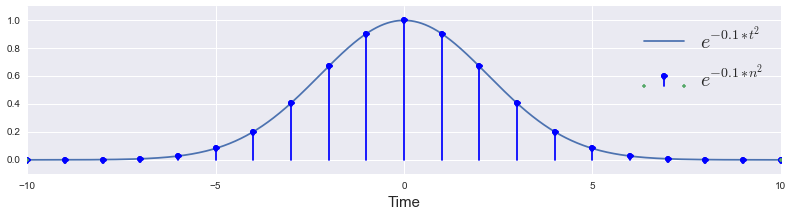
\includegraphics[width=\textwidth]{figs/stem-plot.png}
\caption{Continuous-time and discrete-time signals} \label{fig:ch1_stem}
\end{figure}

\vspace{0.2cm}
{\small \color{black!70!} \noindent\textbf{Note}: Although these signals are called continuous-time and discrete-time, there is not restriction on the choice of the independent variable - it can be time, space, etc. The name 'time' is used in the naming convention as time signals are the most commonly encountered signals in practice.}

In the above example, the discrete-time signal was obtained by selecting the values of the continuous-time signal at specific (equidistant) time points. This is the process of \textit{sampling}, which we will be dealt in detail in Chapter 4.

\begin{figure}[h]
\centering
    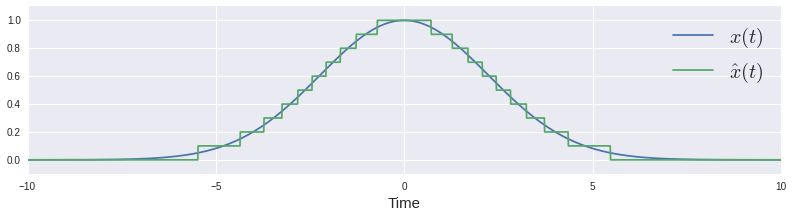
\includegraphics[width=\textwidth]{figs/quantization-plot.png}
\caption{Continuous-time and discrete-time signals} \label{fig:ch1_quant}
\end{figure}

\subsection{Continuous-valued and Discrete-valued Signals}
The previous classification was based on the discretiation of the indepndent variable, while the current classification is based on the dsicretization of the dependent variable, i.e. the values assumed by a signal for different values of its independent variable. When a signal can take  any value in a continuous interval in $\mathbb{R}$, it is called a \textit{continuous-valued} signal, while a \textit{discrete-valued} signal can only take on specific values from a set of values. In the case of \textit{discrete-valued} signals, the set of values the signal can take are usually equidistant. An example of a continuous-valued $\left(x\left(t\right)\right)$ and discrete-valued $\left(\hat{x}\left(t\right)\right)$ signals are shown in the following figure.

In the above example, the $\hat{x}\left(t\right)$ is the discrete-valued version of $x\left(t\right)$, and it can only take on values in the set $\{\dotsc, -0.2, -0.1, 0, 0.1, 0.2, \dotsc\}$. The conversion of $x\left(t\right)$ to $\hat{x}\left(t\right)$ is called \textit{quantization}, which will be discussed in a later chapter.

The last two classifications can be combined to have four possible combinations of signals:
\begin{itemize}
    \item \textbf{Continuous-time continuous-valued signals}: Both the domain and range can take on continous values.
    \item \textbf{Continuous-time discrete-valued signals}: Domain takes on continuous values, while the range can only take on specific discrete values.
    \item \textbf{Discrete-time continuous-valued signals}: Domain taken on values from a discrete set, while the range is continuous
    \item \textbf{Discrete-time discrete-valued signals}: Both the domain and the range take on discrete values.
\end{itemize}

These four cases are demonstrated in the following four figures.

\begin{figure}[h]
\centering
    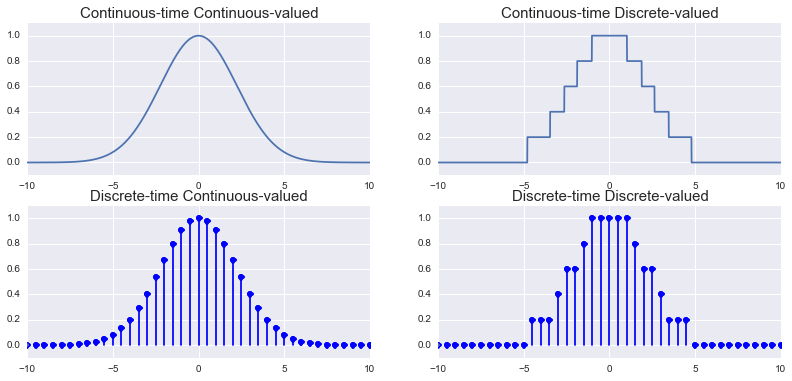
\includegraphics[width=\textwidth]{figs/full-classify.png}
\caption{Continuous-time and discrete-time signals} \label{fig:ch2_full}
\end{figure}

\subsection{Even and Odd Signals}
This classification is based on the symmerty of signals about the vertical axis. A continous-time signal $x\left(t\right)$ is called even, if 
\[ x\left(t\right) = x\left(-t\right), \,\, \forall t \]

The signal $x\left(t\right)$ is called odd, if
\[ x\left(t\right) = -x\left(-t\right), \,\, \forall t \]

Even signals are \textit{symmertric} about the vertical axis (about the point $t = 0$), while odd signals are \textit{antisymmetric} about the vertical axis. This classification also applied to discrete-time signals.

An interesting property of signals is that any signal $x\left(t\right)$ (even, odd or neigther) can be decomposed into an even and odd component. Lets us supposed that $x\left(t\right)$ can be decomposed into an even $x_{e}\left(t\right)$ and an odd $x_{o}\left(t\right)$ component.
\[ x\left(t\right) = x_{e}\left(t\right) + x_{o}\left(t\right) \implies x\left(-t\right) = x_{e}\left(t\right) - x_{o}\left(t\right) \]

Thus,
\[ x_{e}\left(t\right) = \frac{x\left(t\right) + x\left(-t\right)}{2} \,\,\, \& \,\,\, x_{o}\left(t\right) = \frac{x\left(t\right) - x\left(-t\right)}{2} \]

\subsection{Periodic and Non-periodic Signals}
A periodic signal is one that repeats itself after a fixed finite value of time (or the corresponding independent variable), i.e. if the continuous-time $x\left(\right)$ is periodic, then

\[ x\left(t\right) = x\left(t + T\right), \,\,\, \forall t \]

where $T$ is a positive constant. If $T$ is the smallest positive value for which the above relationship is satisfied, then $T$ is called the fundamental period of the signal, and the following is also true.

\[ x\left(t\right) = x\left(t + T\right) = x\left(t + 2T\right)  = x\left(t + 3T\right) \dotsc , \,\,\, \forall t \]

The inverse of $T$ is called the fundamental frequency.

Any signal that does not satisfy the above condition is called an \textit{aperiodic} or \textit{non-periodic} signal.

In the case of a discrete-time signal $x\left[n\right]$, the following condition must be satisfied for the signal to be periodic,
\[ x\left[n\right] = x\left[n + N\right], \,\,\, \forall n \in \mathbb{Z} \,\,\, \& \,\,\, N \in \mathbb{Z} \]

The fundamental period of a discrete-time signal must be an integer.

\subsection{Deterministic and Stochastic Signals}
All the signals we seen so far have been descriveds through a mathematical expression. Such an expression allows one to completely characterize the signal on the domain over which it is defined. Such signals are termed \textit{deterministic}. The representation of deterministic signals is not limited to mathematical expressions; a table of values or a well-defined rule for its calculation would also do as well. These explicit representations of the signal is known as the \textit{signal model}. Through the signal model, the value of the signal can be be predicted for any value of its arguments in its domain. 

A \textit{stochastic} or \textit{random} signal is one that cannot be represented by an explicit mathematical expression to any reasonable accuracy, or it is exceedingly complicated to do so for any practical purposes. Stochastic signals evolve in an unpredicatable fashion as a functions of its arguments. For example, the EMG signal recorded using surface electrodes from a muscle is a stochastic signal. Unlike deterministic signals, which are ammenable to classical techniques of mathematical analysis, statistical techniques are the main tools for analysing stochastic signals.

\subsection{Energy and Power Signals}
Consider a continuous-time signals $v\left(t\right)$ and $i\left(t\right)$, which represent the voltage across and the current through a resistor $R$, respectively. Then the instantaneous power dissipated in the resistor is,
\[ P\left(t\right) = \frac{v^{2}\left(t\right)}{R} = Ri^{2}\left(t\right) \]

In both cases the power is proportional to the resistance $R$. When the value of the resistance in 1omh, then the instantaneous power takes the same form for both $v\left(t\right)$ and $i\left(t\right)$.

In signal processing, regardless of the type of signal represented by $x\left(t\right)$, the instantaneous power is defined as,
\[ p\left(t\right) = x^{2}\left(t\right) \]

\noindent Thus the total energy in a signal $x\left(t\right), \,\,\, t \in (-\infty, \infty)$ is given by,
\[ E = \int_{-\infty}^{\infty} x^{2}\left(t\right) dt \]

\noindent and the average power is defined as,
\[ P = \lim_{T \to \infty} \frac{1}{T} \int_{-T/2}^{T/2} x^{2}\left(t\right) dt \]

Similar definitions can be given for discrete-time signals $\left(x\left[n\right]\right)$ as well, by replacing the integrals by sums. The total energy in $x\left[n\right]$ is,
\[ E = \sum_{n=-\infty}^{\infty} x^{2}\left[n\right] \]

\noindent And the average power is,
\[ P = \lim_{N \to \infty} \sum_{n=-N}^{N} x^{2}\left[n\right] \]

\noindent Based on these definitions, an \textit{energy} signal is defined as any signal whose total energy $E$ is finite. i.e.
\[ 0 < E < \infty \]

\noindent While a signal is called a \textit{power} signal if its average power is finite.
$$0 < P < \infty$$

Thus, an energy signal has zero time-averaged power, and a power signal have infinite energy. Periodic signals are usually viewed as power signals, while non-periodic signals are viewed as energy signals.

\section{What is a system?}
A system is any physical device or algorithm that performs some operation on a singal to transform it into another signal. Mathematically, systems can be thought of as functions or operators that map a signal to another signal. For example, an amplifier increases the amplitude of a signals, a filter removes components of a signals that are considered unwanted, etc. The following figure show a schematic of a system that takes a signal as its input, processes the signal and provides an output processed signal.

\begin{figure}[h]
\centering
    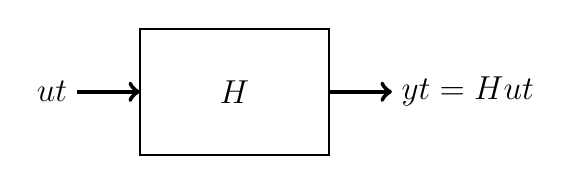
\begin{tikzpicture}[scale=0.8]
        \draw[thick] (0,0) rectangle (3, 2);
        \node at (1.5, 1) {{\large $H$}};
        \draw[ultra thick, ->] (-1, 1) -- (0, 1);
        \node[left] at (-1, 1) {{\large $u\lp t\rp$}};
        \draw[ultra thick, ->] (3, 1) -- (4, 1);
        \node[right] at (4, 1) {{\large $y\lp t\rp = H\lc u\lp t\rp\rc$}};
    \end{tikzpicture}
\caption{Schematic depiction of a system} \label{fig:ch1_system}
\end{figure}

\section{Properites of systems}
Systems are characterized by the nature of the operations that they perform on an input signal. The different classifications of systems, similar to that of singals, are characterized by the type of signals they deal with and the type of opertaions they perform on signals. Instead of presenting the different types of clasifications, like the one done for signals, here present some of the general characteristrics of systems which can be used as a basis for classifying systems.

\subsection{Linearity}
Linearity is an important properpty. All systems we will study and design in this book will be systems that are linear. A system is said to be linear when it satisfies the properties of scaling and superposition. Consider a system $f$ that operates on a set of signals $x_{i}\left(t\right), i \in \{1, 2, \dotsc n\}$ and produces the outputs $y_{i}\left(t\right)$ respectively, i.e.
\[ y_{i}\left(t\right) = f\left(x_{i}\left(t\right)\right), \, i \in \{1, 2, \dotsc n\} \]
Then, the system $f$ is linear if and only if the following is true.
\[ f\left(\sum_{i} a_{i}x_{i}\left(t\right)\right) = \sum_{i}a_{i}y_{i}\left(t\right) \]
where, $a_i$s are some arbitrary constants. The scaling and superpostion properties are both contained in the previous statement. 

\textit{Scaling} refers to the multiplication of the input signals by an arbitrary constant $a$ results in the an output that is also equally scaled (multiplied by $a$), i.e. 
\[ f: x_1 \mapsto y_1 \implies ax_1 \mapsto ay_1 \]

The principle of superposition says that if we know the output of a linear system to a set of inputs $x_{i}, i \in \{1, 2, 3, \dotsc n\}$, then the output of the system to the sum of these inputs is simply the sum of the outputs corresponding to these individual inputs. i.e.
\[ f: x_{i} \mapsto y_{i} \implies \sum_{i} x_{i} \mapsto \sum_{i} y_{i} \]

Linearity is a very important property, and all systems that we will analyze and design in the rest of this book will be based on the linearity assumption, i.e. linear systems. Any system that does not satisfy the scaling and superposition properties are known as \textit{non-linear} systems. Almost all real systems are non-linear, but it will be convenient to assume that they are linear (or approximately linear) in order to use the tools of signal processing and systems theory.

\subsection{Memory}
The property of memory is easy to understand in the context of a system that operates on time-domain signals. A system is said to have memory if its behavior depends on the past (and may be future) values of its input. On the contrary, it is said to be memoryless if its behavior only depends on the current values of its input.

\begin{figure}\centering
    \subcaptionbox{System without memory.}{
    \begin{tikzpicture}[scale=0.9, transform shape]
        \path (0,0) coordinate (ref_gnd);
        \draw
            (ref_gnd) to[american current source={\Large  $i\lp t\rp$}] ++(0, 2.75) -- (0, 2.75)
            (0, 2.75) -- (3, 2.75)
            % (0, 2.75) -- (0, 2.75) to[R=\(R_1\)] ++(2, 0)
            (2.0, 2.75) to[R=\(R\)] ++(0, -2.75) -- (ref_gnd)
            (ref_gnd) -- (3.0, 0) node[] {$\bullet$}
            (2, 2.75) -- (3.0, 2.75) node[] {$\bullet$};
        \draw[-latex] (3.5, 0.95) node[] {} -- (3.5, 0.1) node[] {};
        \draw[-latex] (3.5, 1.65) node[below] {\Large $v\ct{t}$} -- (3.5, 2.65) node[] {};
      \end{tikzpicture}} \quad 
    \subcaptionbox{System with memory.}{
    \begin{tikzpicture}[scale=0.9, transform shape]
        \path (0,0) coordinate (ref_gnd);
        \draw
            (ref_gnd) to[american current source={\Large $i\lp t\rp$}] ++(0, 2.75) -- (0, 2.75)
            (0, 2.75) -- (3, 2.75)
            % (0, 2.75) -- (0, 2.75) to[R=\(R\)] ++(2, 0)
            (2.0, 2.75) to[C=\(C\)] ++(0, -2.75) -- (ref_gnd)
            (ref_gnd) -- (3.0, 0) node[] {$\bullet$}
            (2, 2.75) -- (3.0, 2.75) node[] {$\bullet$};
        \draw[-latex] (3.75, 0.95) node[] {} -- (3.75, 0.1) node[] {};
        \draw[-latex] (3.75, 1.65) node[below] {\Large $v\ct{t}$} -- (3.75, 2.65) node[] {};
      \end{tikzpicture}}
    \caption{Simple examples of electrical systems with and without memory.}
    \label{fig:system_memory}
\end{figure}

The followings are the input-output relationships for the two systems that are shown in the above Fig. \ref{fig:system_memory}. The input to both these systems is a current source $i\ct{t}$, and their corresponding outputs $v\ct{t}$ are the voltages across the resistor $R$, and the capacitor $C$.

\subsubsection{Resistor driven by a current source}
The output voltage of this circuit is,
\[ v\left(t\right) = R \times i\left(t\right) \]

\noindent The output at any given time $t$ only depends on the input value at that particular time. The input-output relationship of this system is shown in Fig. \ref{fig:rc_graph}(a).

\subsubsection{Capacitor driven by a current source}
For the capacitor (Fig. \ref{fig:system_memory}), the input-output relationship is slightly more complicated. The relationship between $i\ct{t}$ and $v\ct{t}$ are governed by the following,
\[ v\ct{t} = \frac{1}{C}\int_{-\infty}^{t} i\ct{\tau}d\tau \]

\noindent The output at any given time $t$ depends on the entire history of the input signal $i\ct{t}$ for all time. The input-output relationship of this system is shown in Fig. \ref{fig:rc_graph}(b).

\begin{figure}[h]
\centering
\subcaptionbox{Resistor circuit $\ct{R = 2\Omega}$}{
    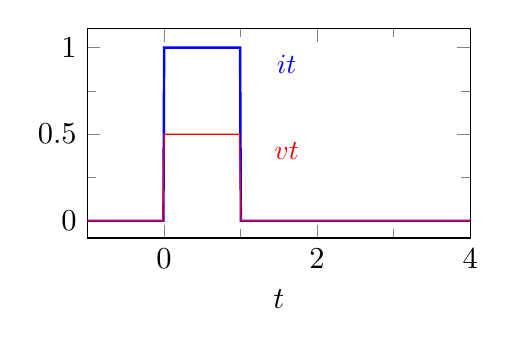
\begin{tikzpicture}[scale=1.1]
        \begin{axis}[xmin=-1,
        xmax=4,
        ymin=-0.1,
        samples=100,
        grid style={line width=.1pt, draw=gray!10},
        major grid style={line width=.2pt,draw=gray!50},
        minor tick num=1,
        xlabel={{$t$}},
        ylabel={},
        title={},
        width=6cm,
        height=4.0cm]
        \addplot[domain=-1:4, blue, thick, samples=500] { x < 0 ? 0 : (x < 1 ? 1: 0)};
        \addplot[domain=-2:8, red, samples=500] { x < 0 ? 0 : (x < 1 ? 0.5: 0)};
    \end{axis}
    \node[blue] at (2.3, 2) {$i\ct{t}$};
    \node[red] at (2.3, 1.0) {$v\ct{t}$};
    \end{tikzpicture}
}
\subcaptionbox{Capacitor circuit $\ct{C = 1.5 F}$}{
    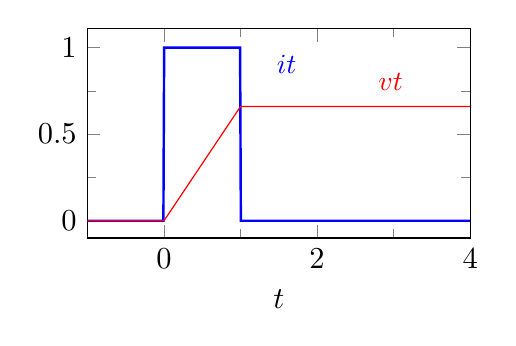
\begin{tikzpicture}[scale=1.1]
        \begin{axis}[xmin=-1,
        xmax=4,
        ymin=-0.1,
        samples=100,
        grid style={line width=.1pt, draw=gray!10},
        major grid style={line width=.2pt,draw=gray!50},
        minor tick num=1,
        xlabel={{$t$}},
        ylabel={},
        title={},
        width=6cm,
        height=4.0cm]
        \addplot[domain=-1:4, blue, thick, samples=500] { x < 0 ? 0 : (x < 1 ? 1: 0)};
        \addplot[domain=-2:8, red, samples=500] { x < 0 ? 0 : (x < 1 ? 0.66 * x: 0.66)};
    \end{axis}
    \node[blue] at (2.3, 2) {$i\ct{t}$};
    \node[red] at (3.5, 1.8) {$v\ct{t}$};
    \end{tikzpicture}
}
\caption{Input output relationship of a system (a) without and (b) with memory.} \label{fig:rc_graph}
\end{figure}

\subsection{Causality}
A system is said to be causal if its output depends only on the present and past values of its inputs, and not on the future values. While, a non-causal system's output depends also on the future values of the input signal. Causality and non-causality are purely based on what is considered the present. The choice of what is the present is fixed for systems that operate in real-time. For example, a filter t that is operating in real-time is strictly causal. However, a system that works off-line on stored data (non-real time) is free to define its present, and thus use data from the future to generate its output.

\subsection{Time-invariance}
Time-invariance property deals with whether or not a system changes over time. This change over time is characterized by the input-output relationship of the system. A system is said to time-invariant if its input-output relationship does not change with time, i.e. one get the same output from the system for a given input independent of whether the input was applied now, 10 minutes earlier or a year from now. Any system where this property does not hold is termed as time-variant. Time-invariance is another property that we will assume in the systems that we analyze and design in the upcoming chapters.

\subsection{Stability}
Stability refers to the property of a system to produce limited output when provided with finite input. Such systems are called stable system in the \textit{bounded-input bounded-output (BIBO)} sense. Systems that do not satisfy the BIBO criteria are called unstable systems.

\subsection{Invertibility}
A system is said to invertible if an inverse of this system can be constructed, i.e. if a system $f$ maps $x\left(t\right)$ to $y\left(t\right)$, then the inverse of the system will map $y\left(t\right)$ to $x\left(t\right)$.
